\documentclass[12pt,a4paper]{article}

\usepackage[a4paper,width=160mm,top=25mm,bottom=25mm]{geometry}

\usepackage{fancyhdr}
\pagestyle{fancy}
\fancyhf{}
\fancyhead[EL]{\nouppercase\leftmark}
\fancyhead[OR]{\nouppercase\rightmark}
\fancyhead[ER,OL]{\thepage}

\usepackage{url}
\usepackage[hidelinks]{hyperref}

\renewcommand{\linethickness}{0.05em}
\usepackage[brazil]{babel}   
\usepackage{titlesec}
\newcommand{\sectionbreak}{\clearpage}


\title{Processando a Informação: um livro prático de programação independente de linguagem 
\\\large\vspace{2cm}
Rogério Perino de Oliveira Neves 
\\\vspace{5mm}
Francisco de Assis Zampirolli
\\\large\vspace{2cm}
EDUFABC
\\ \url{editora.ufabc.edu.br}
\\\Huge\vspace{3cm}
Notas de Aulas inspiradas no livro
\\\Large\vspace{1cm}
Utilizando a(s) Linguagem(ns) de Programação: 
\\\Huge\vspace{1cm}
C
\\\large\vspace{1cm}
Exemplos adaptados para Correção Automática no Moodle+VPL
\vspace{2cm}}
\author{Francisco de Assis Zampirolli\vspace{1cm}}


    \usepackage[breakable]{tcolorbox}
    \usepackage{parskip} % Stop auto-indenting (to mimic markdown behaviour)
    

    % Basic figure setup, for now with no caption control since it's done
    % automatically by Pandoc (which extracts ![](path) syntax from Markdown).
    \usepackage{graphicx}
    % Maintain compatibility with old templates. Remove in nbconvert 6.0
    \let\Oldincludegraphics\includegraphics
    % Ensure that by default, figures have no caption (until we provide a
    % proper Figure object with a Caption API and a way to capture that
    % in the conversion process - todo).
    \usepackage{caption}
    \DeclareCaptionFormat{nocaption}{}
    \captionsetup{format=nocaption,aboveskip=0pt,belowskip=0pt}

    \usepackage{float}
    \floatplacement{figure}{H} % forces figures to be placed at the correct location
    \usepackage{xcolor} % Allow colors to be defined
    \usepackage{enumerate} % Needed for markdown enumerations to work
    \usepackage{geometry} % Used to adjust the document margins
    \usepackage{amsmath} % Equations
    \usepackage{amssymb} % Equations
    \usepackage{textcomp} % defines textquotesingle
    % Hack from http://tex.stackexchange.com/a/47451/13684:
    \AtBeginDocument{%
        \def\PYZsq{\textquotesingle}% Upright quotes in Pygmentized code
    }
    \usepackage{upquote} % Upright quotes for verbatim code
    \usepackage{eurosym} % defines \euro

    \usepackage{iftex}
    \ifPDFTeX
        \usepackage[T1]{fontenc}
        \IfFileExists{alphabeta.sty}{
              \usepackage{alphabeta}
          }{
              \usepackage[mathletters]{ucs}
              \usepackage[utf8x]{inputenc}
          }
    \else
        \usepackage{fontspec}
        \usepackage{unicode-math}
    \fi

    \usepackage{fancyvrb} % verbatim replacement that allows latex
    \usepackage{grffile} % extends the file name processing of package graphics
                         % to support a larger range
    \makeatletter % fix for old versions of grffile with XeLaTeX
    \@ifpackagelater{grffile}{2019/11/01}
    {
      % Do nothing on new versions
    }
    {
      \def\Gread@@xetex#1{%
        \IfFileExists{"\Gin@base".bb}%
        {\Gread@eps{\Gin@base.bb}}%
        {\Gread@@xetex@aux#1}%
      }
    }
    \makeatother
    \usepackage[Export]{adjustbox} % Used to constrain images to a maximum size
    \adjustboxset{max size={0.9\linewidth}{0.9\paperheight}}

    % The hyperref package gives us a pdf with properly built
    % internal navigation ('pdf bookmarks' for the table of contents,
    % internal cross-reference links, web links for URLs, etc.)
    \usepackage{hyperref}
    % The default LaTeX title has an obnoxious amount of whitespace. By default,
    % titling removes some of it. It also provides customization options.
    \usepackage{titling}
    \usepackage{longtable} % longtable support required by pandoc >1.10
    \usepackage{booktabs}  % table support for pandoc > 1.12.2
    \usepackage{array}     % table support for pandoc >= 2.11.3
    \usepackage{calc}      % table minipage width calculation for pandoc >= 2.11.1
    \usepackage[inline]{enumitem} % IRkernel/repr support (it uses the enumerate* environment)
    \usepackage[normalem]{ulem} % ulem is needed to support strikethroughs (\sout)
                                % normalem makes italics be italics, not underlines
    \usepackage{mathrsfs}
    

    
    % Colors for the hyperref package
    \definecolor{urlcolor}{rgb}{0,.145,.698}
    \definecolor{linkcolor}{rgb}{.71,0.21,0.01}
    \definecolor{citecolor}{rgb}{.12,.54,.11}

    % ANSI colors
    \definecolor{ansi-black}{HTML}{3E424D}
    \definecolor{ansi-black-intense}{HTML}{282C36}
    \definecolor{ansi-red}{HTML}{E75C58}
    \definecolor{ansi-red-intense}{HTML}{B22B31}
    \definecolor{ansi-green}{HTML}{00A250}
    \definecolor{ansi-green-intense}{HTML}{007427}
    \definecolor{ansi-yellow}{HTML}{DDB62B}
    \definecolor{ansi-yellow-intense}{HTML}{B27D12}
    \definecolor{ansi-blue}{HTML}{208FFB}
    \definecolor{ansi-blue-intense}{HTML}{0065CA}
    \definecolor{ansi-magenta}{HTML}{D160C4}
    \definecolor{ansi-magenta-intense}{HTML}{A03196}
    \definecolor{ansi-cyan}{HTML}{60C6C8}
    \definecolor{ansi-cyan-intense}{HTML}{258F8F}
    \definecolor{ansi-white}{HTML}{C5C1B4}
    \definecolor{ansi-white-intense}{HTML}{A1A6B2}
    \definecolor{ansi-default-inverse-fg}{HTML}{FFFFFF}
    \definecolor{ansi-default-inverse-bg}{HTML}{000000}

    % common color for the border for error outputs.
    \definecolor{outerrorbackground}{HTML}{FFDFDF}

    % commands and environments needed by pandoc snippets
    % extracted from the output of `pandoc -s`
    \providecommand{\tightlist}{%
      \setlength{\itemsep}{0pt}\setlength{\parskip}{0pt}}
    \DefineVerbatimEnvironment{Highlighting}{Verbatim}{commandchars=\\\{\}}
    % Add ',fontsize=\small' for more characters per line
    \newenvironment{Shaded}{}{}
    \newcommand{\KeywordTok}[1]{\textcolor[rgb]{0.00,0.44,0.13}{\textbf{{#1}}}}
    \newcommand{\DataTypeTok}[1]{\textcolor[rgb]{0.56,0.13,0.00}{{#1}}}
    \newcommand{\DecValTok}[1]{\textcolor[rgb]{0.25,0.63,0.44}{{#1}}}
    \newcommand{\BaseNTok}[1]{\textcolor[rgb]{0.25,0.63,0.44}{{#1}}}
    \newcommand{\FloatTok}[1]{\textcolor[rgb]{0.25,0.63,0.44}{{#1}}}
    \newcommand{\CharTok}[1]{\textcolor[rgb]{0.25,0.44,0.63}{{#1}}}
    \newcommand{\StringTok}[1]{\textcolor[rgb]{0.25,0.44,0.63}{{#1}}}
    \newcommand{\CommentTok}[1]{\textcolor[rgb]{0.38,0.63,0.69}{\textit{{#1}}}}
    \newcommand{\OtherTok}[1]{\textcolor[rgb]{0.00,0.44,0.13}{{#1}}}
    \newcommand{\AlertTok}[1]{\textcolor[rgb]{1.00,0.00,0.00}{\textbf{{#1}}}}
    \newcommand{\FunctionTok}[1]{\textcolor[rgb]{0.02,0.16,0.49}{{#1}}}
    \newcommand{\RegionMarkerTok}[1]{{#1}}
    \newcommand{\ErrorTok}[1]{\textcolor[rgb]{1.00,0.00,0.00}{\textbf{{#1}}}}
    \newcommand{\NormalTok}[1]{{#1}}

    % Additional commands for more recent versions of Pandoc
    \newcommand{\ConstantTok}[1]{\textcolor[rgb]{0.53,0.00,0.00}{{#1}}}
    \newcommand{\SpecialCharTok}[1]{\textcolor[rgb]{0.25,0.44,0.63}{{#1}}}
    \newcommand{\VerbatimStringTok}[1]{\textcolor[rgb]{0.25,0.44,0.63}{{#1}}}
    \newcommand{\SpecialStringTok}[1]{\textcolor[rgb]{0.73,0.40,0.53}{{#1}}}
    \newcommand{\ImportTok}[1]{{#1}}
    \newcommand{\DocumentationTok}[1]{\textcolor[rgb]{0.73,0.13,0.13}{\textit{{#1}}}}
    \newcommand{\AnnotationTok}[1]{\textcolor[rgb]{0.38,0.63,0.69}{\textbf{\textit{{#1}}}}}
    \newcommand{\CommentVarTok}[1]{\textcolor[rgb]{0.38,0.63,0.69}{\textbf{\textit{{#1}}}}}
    \newcommand{\VariableTok}[1]{\textcolor[rgb]{0.10,0.09,0.49}{{#1}}}
    \newcommand{\ControlFlowTok}[1]{\textcolor[rgb]{0.00,0.44,0.13}{\textbf{{#1}}}}
    \newcommand{\OperatorTok}[1]{\textcolor[rgb]{0.40,0.40,0.40}{{#1}}}
    \newcommand{\BuiltInTok}[1]{{#1}}
    \newcommand{\ExtensionTok}[1]{{#1}}
    \newcommand{\PreprocessorTok}[1]{\textcolor[rgb]{0.74,0.48,0.00}{{#1}}}
    \newcommand{\AttributeTok}[1]{\textcolor[rgb]{0.49,0.56,0.16}{{#1}}}
    \newcommand{\InformationTok}[1]{\textcolor[rgb]{0.38,0.63,0.69}{\textbf{\textit{{#1}}}}}
    \newcommand{\WarningTok}[1]{\textcolor[rgb]{0.38,0.63,0.69}{\textbf{\textit{{#1}}}}}


    % Define a nice break command that doesn't care if a line doesn't already
    % exist.
    \def\br{\hspace*{\fill} \\* }
    % Math Jax compatibility definitions
    \def\gt{>}
    \def\lt{<}
    \let\Oldtex\TeX
    \let\Oldlatex\LaTeX
    \renewcommand{\TeX}{\textrm{\Oldtex}}
    \renewcommand{\LaTeX}{\textrm{\Oldlatex}}
    % Document parameters
    % Document title
    %\title{cap3.part1.c}
    
    
    
    
    
% Pygments definitions
\makeatletter
\def\PY@reset{\let\PY@it=\relax \let\PY@bf=\relax%
    \let\PY@ul=\relax \let\PY@tc=\relax%
    \let\PY@bc=\relax \let\PY@ff=\relax}
\def\PY@tok#1{\csname PY@tok@#1\endcsname}
\def\PY@toks#1+{\ifx\relax#1\empty\else%
    \PY@tok{#1}\expandafter\PY@toks\fi}
\def\PY@do#1{\PY@bc{\PY@tc{\PY@ul{%
    \PY@it{\PY@bf{\PY@ff{#1}}}}}}}
\def\PY#1#2{\PY@reset\PY@toks#1+\relax+\PY@do{#2}}

\@namedef{PY@tok@w}{\def\PY@tc##1{\textcolor[rgb]{0.73,0.73,0.73}{##1}}}
\@namedef{PY@tok@c}{\let\PY@it=\textit\def\PY@tc##1{\textcolor[rgb]{0.24,0.48,0.48}{##1}}}
\@namedef{PY@tok@cp}{\def\PY@tc##1{\textcolor[rgb]{0.61,0.40,0.00}{##1}}}
\@namedef{PY@tok@k}{\let\PY@bf=\textbf\def\PY@tc##1{\textcolor[rgb]{0.00,0.50,0.00}{##1}}}
\@namedef{PY@tok@kp}{\def\PY@tc##1{\textcolor[rgb]{0.00,0.50,0.00}{##1}}}
\@namedef{PY@tok@kt}{\def\PY@tc##1{\textcolor[rgb]{0.69,0.00,0.25}{##1}}}
\@namedef{PY@tok@o}{\def\PY@tc##1{\textcolor[rgb]{0.40,0.40,0.40}{##1}}}
\@namedef{PY@tok@ow}{\let\PY@bf=\textbf\def\PY@tc##1{\textcolor[rgb]{0.67,0.13,1.00}{##1}}}
\@namedef{PY@tok@nb}{\def\PY@tc##1{\textcolor[rgb]{0.00,0.50,0.00}{##1}}}
\@namedef{PY@tok@nf}{\def\PY@tc##1{\textcolor[rgb]{0.00,0.00,1.00}{##1}}}
\@namedef{PY@tok@nc}{\let\PY@bf=\textbf\def\PY@tc##1{\textcolor[rgb]{0.00,0.00,1.00}{##1}}}
\@namedef{PY@tok@nn}{\let\PY@bf=\textbf\def\PY@tc##1{\textcolor[rgb]{0.00,0.00,1.00}{##1}}}
\@namedef{PY@tok@ne}{\let\PY@bf=\textbf\def\PY@tc##1{\textcolor[rgb]{0.80,0.25,0.22}{##1}}}
\@namedef{PY@tok@nv}{\def\PY@tc##1{\textcolor[rgb]{0.10,0.09,0.49}{##1}}}
\@namedef{PY@tok@no}{\def\PY@tc##1{\textcolor[rgb]{0.53,0.00,0.00}{##1}}}
\@namedef{PY@tok@nl}{\def\PY@tc##1{\textcolor[rgb]{0.46,0.46,0.00}{##1}}}
\@namedef{PY@tok@ni}{\let\PY@bf=\textbf\def\PY@tc##1{\textcolor[rgb]{0.44,0.44,0.44}{##1}}}
\@namedef{PY@tok@na}{\def\PY@tc##1{\textcolor[rgb]{0.41,0.47,0.13}{##1}}}
\@namedef{PY@tok@nt}{\let\PY@bf=\textbf\def\PY@tc##1{\textcolor[rgb]{0.00,0.50,0.00}{##1}}}
\@namedef{PY@tok@nd}{\def\PY@tc##1{\textcolor[rgb]{0.67,0.13,1.00}{##1}}}
\@namedef{PY@tok@s}{\def\PY@tc##1{\textcolor[rgb]{0.73,0.13,0.13}{##1}}}
\@namedef{PY@tok@sd}{\let\PY@it=\textit\def\PY@tc##1{\textcolor[rgb]{0.73,0.13,0.13}{##1}}}
\@namedef{PY@tok@si}{\let\PY@bf=\textbf\def\PY@tc##1{\textcolor[rgb]{0.64,0.35,0.47}{##1}}}
\@namedef{PY@tok@se}{\let\PY@bf=\textbf\def\PY@tc##1{\textcolor[rgb]{0.67,0.36,0.12}{##1}}}
\@namedef{PY@tok@sr}{\def\PY@tc##1{\textcolor[rgb]{0.64,0.35,0.47}{##1}}}
\@namedef{PY@tok@ss}{\def\PY@tc##1{\textcolor[rgb]{0.10,0.09,0.49}{##1}}}
\@namedef{PY@tok@sx}{\def\PY@tc##1{\textcolor[rgb]{0.00,0.50,0.00}{##1}}}
\@namedef{PY@tok@m}{\def\PY@tc##1{\textcolor[rgb]{0.40,0.40,0.40}{##1}}}
\@namedef{PY@tok@gh}{\let\PY@bf=\textbf\def\PY@tc##1{\textcolor[rgb]{0.00,0.00,0.50}{##1}}}
\@namedef{PY@tok@gu}{\let\PY@bf=\textbf\def\PY@tc##1{\textcolor[rgb]{0.50,0.00,0.50}{##1}}}
\@namedef{PY@tok@gd}{\def\PY@tc##1{\textcolor[rgb]{0.63,0.00,0.00}{##1}}}
\@namedef{PY@tok@gi}{\def\PY@tc##1{\textcolor[rgb]{0.00,0.52,0.00}{##1}}}
\@namedef{PY@tok@gr}{\def\PY@tc##1{\textcolor[rgb]{0.89,0.00,0.00}{##1}}}
\@namedef{PY@tok@ge}{\let\PY@it=\textit}
\@namedef{PY@tok@gs}{\let\PY@bf=\textbf}
\@namedef{PY@tok@gp}{\let\PY@bf=\textbf\def\PY@tc##1{\textcolor[rgb]{0.00,0.00,0.50}{##1}}}
\@namedef{PY@tok@go}{\def\PY@tc##1{\textcolor[rgb]{0.44,0.44,0.44}{##1}}}
\@namedef{PY@tok@gt}{\def\PY@tc##1{\textcolor[rgb]{0.00,0.27,0.87}{##1}}}
\@namedef{PY@tok@err}{\def\PY@bc##1{{\setlength{\fboxsep}{\string -\fboxrule}\fcolorbox[rgb]{1.00,0.00,0.00}{1,1,1}{\strut ##1}}}}
\@namedef{PY@tok@kc}{\let\PY@bf=\textbf\def\PY@tc##1{\textcolor[rgb]{0.00,0.50,0.00}{##1}}}
\@namedef{PY@tok@kd}{\let\PY@bf=\textbf\def\PY@tc##1{\textcolor[rgb]{0.00,0.50,0.00}{##1}}}
\@namedef{PY@tok@kn}{\let\PY@bf=\textbf\def\PY@tc##1{\textcolor[rgb]{0.00,0.50,0.00}{##1}}}
\@namedef{PY@tok@kr}{\let\PY@bf=\textbf\def\PY@tc##1{\textcolor[rgb]{0.00,0.50,0.00}{##1}}}
\@namedef{PY@tok@bp}{\def\PY@tc##1{\textcolor[rgb]{0.00,0.50,0.00}{##1}}}
\@namedef{PY@tok@fm}{\def\PY@tc##1{\textcolor[rgb]{0.00,0.00,1.00}{##1}}}
\@namedef{PY@tok@vc}{\def\PY@tc##1{\textcolor[rgb]{0.10,0.09,0.49}{##1}}}
\@namedef{PY@tok@vg}{\def\PY@tc##1{\textcolor[rgb]{0.10,0.09,0.49}{##1}}}
\@namedef{PY@tok@vi}{\def\PY@tc##1{\textcolor[rgb]{0.10,0.09,0.49}{##1}}}
\@namedef{PY@tok@vm}{\def\PY@tc##1{\textcolor[rgb]{0.10,0.09,0.49}{##1}}}
\@namedef{PY@tok@sa}{\def\PY@tc##1{\textcolor[rgb]{0.73,0.13,0.13}{##1}}}
\@namedef{PY@tok@sb}{\def\PY@tc##1{\textcolor[rgb]{0.73,0.13,0.13}{##1}}}
\@namedef{PY@tok@sc}{\def\PY@tc##1{\textcolor[rgb]{0.73,0.13,0.13}{##1}}}
\@namedef{PY@tok@dl}{\def\PY@tc##1{\textcolor[rgb]{0.73,0.13,0.13}{##1}}}
\@namedef{PY@tok@s2}{\def\PY@tc##1{\textcolor[rgb]{0.73,0.13,0.13}{##1}}}
\@namedef{PY@tok@sh}{\def\PY@tc##1{\textcolor[rgb]{0.73,0.13,0.13}{##1}}}
\@namedef{PY@tok@s1}{\def\PY@tc##1{\textcolor[rgb]{0.73,0.13,0.13}{##1}}}
\@namedef{PY@tok@mb}{\def\PY@tc##1{\textcolor[rgb]{0.40,0.40,0.40}{##1}}}
\@namedef{PY@tok@mf}{\def\PY@tc##1{\textcolor[rgb]{0.40,0.40,0.40}{##1}}}
\@namedef{PY@tok@mh}{\def\PY@tc##1{\textcolor[rgb]{0.40,0.40,0.40}{##1}}}
\@namedef{PY@tok@mi}{\def\PY@tc##1{\textcolor[rgb]{0.40,0.40,0.40}{##1}}}
\@namedef{PY@tok@il}{\def\PY@tc##1{\textcolor[rgb]{0.40,0.40,0.40}{##1}}}
\@namedef{PY@tok@mo}{\def\PY@tc##1{\textcolor[rgb]{0.40,0.40,0.40}{##1}}}
\@namedef{PY@tok@ch}{\let\PY@it=\textit\def\PY@tc##1{\textcolor[rgb]{0.24,0.48,0.48}{##1}}}
\@namedef{PY@tok@cm}{\let\PY@it=\textit\def\PY@tc##1{\textcolor[rgb]{0.24,0.48,0.48}{##1}}}
\@namedef{PY@tok@cpf}{\let\PY@it=\textit\def\PY@tc##1{\textcolor[rgb]{0.24,0.48,0.48}{##1}}}
\@namedef{PY@tok@c1}{\let\PY@it=\textit\def\PY@tc##1{\textcolor[rgb]{0.24,0.48,0.48}{##1}}}
\@namedef{PY@tok@cs}{\let\PY@it=\textit\def\PY@tc##1{\textcolor[rgb]{0.24,0.48,0.48}{##1}}}

\def\PYZbs{\char`\\}
\def\PYZus{\char`\_}
\def\PYZob{\char`\{}
\def\PYZcb{\char`\}}
\def\PYZca{\char`\^}
\def\PYZam{\char`\&}
\def\PYZlt{\char`\<}
\def\PYZgt{\char`\>}
\def\PYZsh{\char`\#}
\def\PYZpc{\char`\%}
\def\PYZdl{\char`\$}
\def\PYZhy{\char`\-}
\def\PYZsq{\char`\'}
\def\PYZdq{\char`\"}
\def\PYZti{\char`\~}
% for compatibility with earlier versions
\def\PYZat{@}
\def\PYZlb{[}
\def\PYZrb{]}
\makeatother


    % For linebreaks inside Verbatim environment from package fancyvrb.
    \makeatletter
        \newbox\Wrappedcontinuationbox
        \newbox\Wrappedvisiblespacebox
        \newcommand*\Wrappedvisiblespace {\textcolor{red}{\textvisiblespace}}
        \newcommand*\Wrappedcontinuationsymbol {\textcolor{red}{\llap{\tiny$\m@th\hookrightarrow$}}}
        \newcommand*\Wrappedcontinuationindent {3ex }
        \newcommand*\Wrappedafterbreak {\kern\Wrappedcontinuationindent\copy\Wrappedcontinuationbox}
        % Take advantage of the already applied Pygments mark-up to insert
        % potential linebreaks for TeX processing.
        %        {, <, #, %, $, ' and ": go to next line.
        %        _, }, ^, &, >, - and ~: stay at end of broken line.
        % Use of \textquotesingle for straight quote.
        \newcommand*\Wrappedbreaksatspecials {%
            \def\PYGZus{\discretionary{\char`\_}{\Wrappedafterbreak}{\char`\_}}%
            \def\PYGZob{\discretionary{}{\Wrappedafterbreak\char`\{}{\char`\{}}%
            \def\PYGZcb{\discretionary{\char`\}}{\Wrappedafterbreak}{\char`\}}}%
            \def\PYGZca{\discretionary{\char`\^}{\Wrappedafterbreak}{\char`\^}}%
            \def\PYGZam{\discretionary{\char`\&}{\Wrappedafterbreak}{\char`\&}}%
            \def\PYGZlt{\discretionary{}{\Wrappedafterbreak\char`\<}{\char`\<}}%
            \def\PYGZgt{\discretionary{\char`\>}{\Wrappedafterbreak}{\char`\>}}%
            \def\PYGZsh{\discretionary{}{\Wrappedafterbreak\char`\#}{\char`\#}}%
            \def\PYGZpc{\discretionary{}{\Wrappedafterbreak\char`\%}{\char`\%}}%
            \def\PYGZdl{\discretionary{}{\Wrappedafterbreak\char`\$}{\char`\$}}%
            \def\PYGZhy{\discretionary{\char`\-}{\Wrappedafterbreak}{\char`\-}}%
            \def\PYGZsq{\discretionary{}{\Wrappedafterbreak\textquotesingle}{\textquotesingle}}%
            \def\PYGZdq{\discretionary{}{\Wrappedafterbreak\char`\"}{\char`\"}}%
            \def\PYGZti{\discretionary{\char`\~}{\Wrappedafterbreak}{\char`\~}}%
        }
        % Some characters . , ; ? ! / are not pygmentized.
        % This macro makes them "active" and they will insert potential linebreaks
        \newcommand*\Wrappedbreaksatpunct {%
            \lccode`\~`\.\lowercase{\def~}{\discretionary{\hbox{\char`\.}}{\Wrappedafterbreak}{\hbox{\char`\.}}}%
            \lccode`\~`\,\lowercase{\def~}{\discretionary{\hbox{\char`\,}}{\Wrappedafterbreak}{\hbox{\char`\,}}}%
            \lccode`\~`\;\lowercase{\def~}{\discretionary{\hbox{\char`\;}}{\Wrappedafterbreak}{\hbox{\char`\;}}}%
            \lccode`\~`\:\lowercase{\def~}{\discretionary{\hbox{\char`\:}}{\Wrappedafterbreak}{\hbox{\char`\:}}}%
            \lccode`\~`\?\lowercase{\def~}{\discretionary{\hbox{\char`\?}}{\Wrappedafterbreak}{\hbox{\char`\?}}}%
            \lccode`\~`\!\lowercase{\def~}{\discretionary{\hbox{\char`\!}}{\Wrappedafterbreak}{\hbox{\char`\!}}}%
            \lccode`\~`\/\lowercase{\def~}{\discretionary{\hbox{\char`\/}}{\Wrappedafterbreak}{\hbox{\char`\/}}}%
            \catcode`\.\active
            \catcode`\,\active
            \catcode`\;\active
            \catcode`\:\active
            \catcode`\?\active
            \catcode`\!\active
            \catcode`\/\active
            \lccode`\~`\~
        }
    \makeatother

    \let\OriginalVerbatim=\Verbatim
    \makeatletter
    \renewcommand{\Verbatim}[1][1]{%
        %\parskip\z@skip
        \sbox\Wrappedcontinuationbox {\Wrappedcontinuationsymbol}%
        \sbox\Wrappedvisiblespacebox {\FV@SetupFont\Wrappedvisiblespace}%
        \def\FancyVerbFormatLine ##1{\hsize\linewidth
            \vtop{\raggedright\hyphenpenalty\z@\exhyphenpenalty\z@
                \doublehyphendemerits\z@\finalhyphendemerits\z@
                \strut ##1\strut}%
        }%
        % If the linebreak is at a space, the latter will be displayed as visible
        % space at end of first line, and a continuation symbol starts next line.
        % Stretch/shrink are however usually zero for typewriter font.
        \def\FV@Space {%
            \nobreak\hskip\z@ plus\fontdimen3\font minus\fontdimen4\font
            \discretionary{\copy\Wrappedvisiblespacebox}{\Wrappedafterbreak}
            {\kern\fontdimen2\font}%
        }%

        % Allow breaks at special characters using \PYG... macros.
        \Wrappedbreaksatspecials
        % Breaks at punctuation characters . , ; ? ! and / need catcode=\active
        \OriginalVerbatim[#1,codes*=\Wrappedbreaksatpunct]%
    }
    \makeatother

    % Exact colors from NB
    \definecolor{incolor}{HTML}{303F9F}
    \definecolor{outcolor}{HTML}{D84315}
    \definecolor{cellborder}{HTML}{CFCFCF}
    \definecolor{cellbackground}{HTML}{F7F7F7}

    % prompt
    \makeatletter
    \newcommand{\boxspacing}{\kern\kvtcb@left@rule\kern\kvtcb@boxsep}
    \makeatother
    \newcommand{\prompt}[4]{
        {\ttfamily\llap{{\color{#2}[#3]:\hspace{3pt}#4}}\vspace{-\baselineskip}}
    }
    

    
    % Prevent overflowing lines due to hard-to-break entities
    \sloppy
    % Setup hyperref package
    \hypersetup{
      breaklinks=true,  % so long urls are correctly broken across lines
      colorlinks=true,
      urlcolor=urlcolor,
      linkcolor=linkcolor,
      citecolor=citecolor,
      }
    % Slightly bigger margins than the latex defaults
    
    \geometry{verbose,tmargin=1in,bmargin=1in,lmargin=1in,rmargin=1in}
    
    

\begin{document}
    
    
\clearpage\maketitle
\thispagestyle{empty}
\tableofcontents

    
    

    
    \hypertarget{processando-a-informauxe7uxe3o-cap.-3-desvios-condicionais}{%
\section{Processando a Informação: Cap. 3: Desvios
Condicionais}\label{processando-a-informauxe7uxe3o-cap.-3-desvios-condicionais}}

    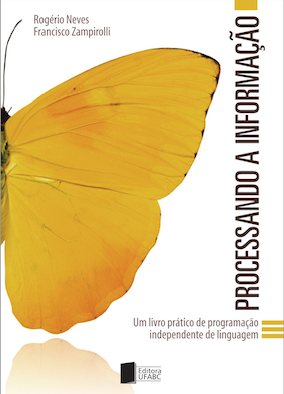
\includegraphics{"figs/Capa_Processando_Informacao.jpg"}

Este caderno (Notebook) é parte complementar \emph{online} do livro
\textbf{\href{https://editora.ufabc.edu.br/matematica-e-ciencias-da-computacao/58-processando-a-informacao}{Processando
a Informação}: um livro prático de programação independente de
linguagem}, que deve ser consultado no caso de dúvidas sobre os temas
apresentados.

\begin{quote}
Este conteúdo pode ser copiado e alterado livremente e foi inspirado
nesse livro.
\end{quote}

    \hypertarget{sumuxe1rio}{%
\subsection{Sumário}\label{sumuxe1rio}}

\begin{itemize}
\tightlist
\item
  Revisão do capítulo anterios
\item
  O que é um desvio condicional?
\item
  Condições com lógica booleana
\item
  Desvios condicionais Simples e Compostos, com Encadeamentos
\item
  Revisão deste capítulo
\item
  Exercícios
\end{itemize}

    \hypertarget{revisuxe3o-do-capuxedtulo-anterior-organizauxe7uxe3o-de-cuxf3digo}{%
\subsection{Revisão do capítulo anterior (Organização de
Código)}\label{revisuxe3o-do-capuxedtulo-anterior-organizauxe7uxe3o-de-cuxf3digo}}

    \begin{itemize}
\item
  No capítulo anterior foram apresentados formas de organização de
  códigos, utilizando comentários, tabulações, escopo de variáveis
  locais e globais, métodos (funções ou procedimentos) e o conceito de
  sistema de informação em partes:

  \begin{quote}
  ENTRADA DE DADOS \(\Rightarrow\) PROCESSAMENTO DA INFORMAÇÃO
  \(\Rightarrow\) SAÍDA
  \end{quote}
\item
  Neste capítulo serão apresentados códigos com desvios condicionais, da
  forma:

  \begin{itemize}
  \tightlist
  \item
    \texttt{se} algo for verdade, \texttt{então}

    \begin{itemize}
    \tightlist
    \item
      faça algo1,
    \end{itemize}
  \item
    \texttt{senão} \# essa parte é opcional

    \begin{itemize}
    \tightlist
    \item
      faça algo2.
    \end{itemize}
  \end{itemize}
\end{itemize}

    \hypertarget{o-que-uxe9-um-desvio-condional}{%
\subsection{O que é um Desvio
Condional?}\label{o-que-uxe9-um-desvio-condional}}

    \begin{itemize}
\item
  O desvio condicional é a mais simples entre as estruturas lógicas não
  sequenciais em lógica de programação e fundamental para o entendimento
  de fluxo de código.
\item
  A analogia básica com o processo de tomada de decisões ocorre quando
  imaginamos um cenário que proporciona duas possíveis alternativas de
  curso:

  \begin{itemize}
  \tightlist
  \item
    Se {[}condição{]} então faça {[}caminho caso verdadeiro{]} senão
    {[}caminho caso falso{]}
  \end{itemize}
\item
  Exemplos:

  \begin{itemize}
  \tightlist
  \item
    Se {[}está chovendo{]} então {[}resolver palavras cruzadas{]} senão
    {[}andar de bicicleta{]}
  \item
    Se {[}é quarta{]} então {[}comer feijoada{]}
  \end{itemize}
\item
  Ver Fluxograma abaixo (também experimente nessa ferramenta
  \emph{online}: \href{https://app.code2flow.com/}{code2flow}, copiando
  e colando o código em vermelho abaixo):
\end{itemize}

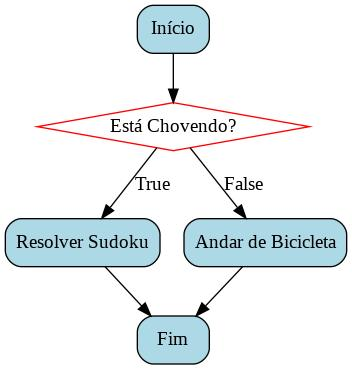
\includegraphics{"figs/flowchartCap3a.jpg"}

    \begin{figure}
\centering
\caption{flowchartCap3a.jpg}
\end{figure}

    \begin{tcolorbox}[breakable, size=fbox, boxrule=1pt, pad at break*=1mm,colback=cellbackground, colframe=cellborder]
\prompt{In}{incolor}{2}{\boxspacing}
\begin{Verbatim}[commandchars=\\\{\}]
\PY{o}{!}apt\PYZhy{}get install graphviz libgraphviz\PYZhy{}dev pkg\PYZhy{}config
\PY{o}{!}pip install txtoflow
\end{Verbatim}
\end{tcolorbox}

    \begin{tcolorbox}[breakable, size=fbox, boxrule=1pt, pad at break*=1mm,colback=cellbackground, colframe=cellborder]
\prompt{In}{incolor}{3}{\boxspacing}
\begin{Verbatim}[commandchars=\\\{\}]
\PY{k+kn}{from} \PY{n+nn}{txtoflow} \PY{k+kn}{import} \PY{n}{txtoflow}

\PY{n}{txtoflow}\PY{o}{.}\PY{n}{generate}\PY{p}{(}
    \PY{l+s+sd}{\PYZsq{}\PYZsq{}\PYZsq{}}
\PY{l+s+sd}{    Início;}
\PY{l+s+sd}{    if (Está Chovendo?) \PYZob{}}
\PY{l+s+sd}{        Resolver Sudoku;}
\PY{l+s+sd}{    \PYZcb{} else \PYZob{}}
\PY{l+s+sd}{        Andar de Bicicleta;}
\PY{l+s+sd}{    \PYZcb{}}
\PY{l+s+sd}{    Fim;}
\PY{l+s+sd}{    \PYZsq{}\PYZsq{}\PYZsq{}}
\PY{p}{)}
\end{Verbatim}
\end{tcolorbox}

    \hypertarget{condiuxe7uxf5es-com-luxf3gica-booleana}{%
\subsection{\texorpdfstring{Condições com Lógica
\emph{Booleana}}{Condições com Lógica Booleana}}\label{condiuxe7uxf5es-com-luxf3gica-booleana}}

    \begin{itemize}
\tightlist
\item
  O resultado de um teste condicional sempre resultará em um valor
  \emph{booleano}, isto é:

  \begin{itemize}
  \tightlist
  \item
    com dois resultados possíveis: \textbf{verdadeiro} ou \textbf{falso}
  \item
    Por convensão: \(True=1\) e \(False=0\)
  \end{itemize}
\item
  Portanto, para condições, sempre usaremos combinações de operadores
  lógicos e relacionais para verificar o estado das variáveis
  verificadas. O seguinte pseudocódigo exemplifica algumas condições:
\end{itemize}

    \begin{verbatim}
se vai chover, então leve um guarda-chuva.

se é feriado, então fique em casa.

se estou atrasado e está chovendo, então chame um taxi.

se minha nota é menor que 5, então fiquei de recuperação.
\end{verbatim}

    \begin{itemize}
\item
  Note que para todas as condições acima, a resposta para a condição é
  sempre: verdadeiro ou falso.
\item
  Caso a condição seja verdadeira, será executada a operação ou
  operações especificadas na sequência.
\item
  Codificando-se, as condições tomam a forma
  \texttt{se\ (condição)\ \{\ comandos\ \}}, como exemplos:
\end{itemize}

    \begin{verbatim}
se (vai_chover) { leve um guarda-chuva }

se (feriado) { fique em casa }

se (atrasado e chovendo) { chame um taxi }

se (nota<5) { escrever “ficou de Recuperação” }
\end{verbatim}

    Esse código anterior \textbf{fica melhor se usar a organização}
apresentada no capítulo anterior:

    \begin{verbatim}
se (vai_chover) 
  leve um guarda-chuva 

se (feriado) 
  fique em casa 

se (atrasado e chovendo)  
  chame um taxi 

se (nota<5) 
  escrever “ficou de Recuperação” 
\end{verbatim}

    \begin{itemize}
\item
  Observe que foram substituídas as chaves \texttt{\{} e \texttt{\}},
  que definem os \textbf{escopos} das condicionais, pela tabulação.
\item
  Relembrando o Cap. 1 - Fundamentos, podemos usar nas
  \textbf{condicionais}, variáveis \emph{booleanas} e operadores:

  \begin{itemize}
  \tightlist
  \item
    \textbf{relacionais}: ◦ == (é igual a) ◦ != (é diferente de) ◦
    \textgreater{} (é maior que) ◦ \textless{} (é menor que) ◦
    \textgreater= (é maior ou igual a) ◦ \textless= (é menor ou igual a)
  \item
    Além de \textbf{lógicos}: ◦ \&\& (e), \& (e bit-a-bit) ◦
    \textbar\textbar{} (ou), \textbar{} (ou bit a bit) ◦ ! (não lógico
    ou complemento) ◦ \textasciitilde{} (complemento bit-a-bit) ◦ \^{}
    (ou exclusivo `XOR' bit-a-bit) ◦ \textless\textless{} N (shift-left,
    adiciona N zeros à direita do número em binário) ◦
    \textgreater\textgreater{} N (shift-right, elimina N dígitos a
    direita do número em binário)
  \end{itemize}
\end{itemize}

    \begin{itemize}
\item
  Os operadores \textbf{lógicos}, como os \textbf{relacionais}, sempre
  resultarão \textbf{verdadeiro} (V) ou \textbf{falso} (F), porém os
  operandos também são \emph{booleanos}.
\item
  Para as condições contendo AND, OR e XOR (ou exclusivo), as
  \textbf{tabelas verdade} para os dois operandos à esquerda e à
  direita, com valores lógicos representados na primeira linha e
  primeira coluna, são:
\end{itemize}

    \begin{longtable}[]{@{}ccc@{}}
\toprule
\&\& & V & F\tabularnewline
\midrule
\endhead
V & \textbf{V} & F\tabularnewline
F & F & F\tabularnewline
\bottomrule
\end{longtable}

    \begin{longtable}[]{@{}ccc@{}}
\toprule
\textbar\textbar{} & V & F\tabularnewline
\midrule
\endhead
V & V & V\tabularnewline
F & V & \textbf{F}\tabularnewline
\bottomrule
\end{longtable}

    \begin{longtable}[]{@{}ccc@{}}
\toprule
\^{} & V & F\tabularnewline
\midrule
\endhead
V & F & V\tabularnewline
F & V & F\tabularnewline
\bottomrule
\end{longtable}

    \begin{itemize}
\tightlist
\item
  Logo,

  \begin{itemize}
  \tightlist
  \item
    os operandos devem ser ambos verdadeiros para que a operação AND
    retorne verdadeiro,
  \item
    ao menos um deles verdadeiro para que o OR retorne verdadeiro e
  \item
    ambos diferentes para que o XOR (ou exclusivo \texttt{\^{}}) retorne
    verdadeiro.
  \end{itemize}
\end{itemize}

    \begin{itemize}
\item
  Estas expressões, quando combinadas, resultarão sempre em um valor
  \emph{booleano} V ou F, que pode ser então introduzido em um desvio
  condicional visando à realização de um subprograma.
\item
  Por exemplo, usando os valores X=1, Y=2 e Z=4, qual o resultado das
  expressões abaixo?
\end{itemize}

\begin{quote}
\begin{enumerate}
\def\labelenumi{\arabic{enumi}.}
\tightlist
\item
  (X\textgreater0 \&\& Y\textless2)
\item
  (Z\textgreater0 \textbar\textbar{} Z\textless5 \&\& Y==4)
\item
  (X\textgreater\textgreater1 ==0 \textbar\textbar{}
  Y\textless\textless2\textgreater100)
\item
  (X!=0 \&\& Y!=0 \&\& Z\textless0)
\item
  (X=1)
\end{enumerate}
\end{quote}

    \begin{itemize}
\tightlist
\item
  Dada a precedência de operadores estudada anteriormente e a combinação
  apresentada acima, apenas as expressões 2 e 3 resultariam em
  verdadeiro, dado \(Z>0\), assim como \(1>>1\) (\emph{shift} à direita
  uma casa) em binário é 0; são ambas condições suficientes para que o
  resultado seja verdadeiro.
\end{itemize}

    \begin{tcolorbox}[breakable, size=fbox, boxrule=1pt, pad at break*=1mm,colback=cellbackground, colframe=cellborder]
\prompt{In}{incolor}{ }{\boxspacing}
\begin{Verbatim}[commandchars=\\\{\}]
\PY{n}{X}\PY{p}{,} \PY{n}{Y}\PY{p}{,} \PY{n}{Z} \PY{o}{=}\PY{l+m+mi}{1}\PY{p}{,} \PY{l+m+mi}{2}\PY{p}{,} \PY{l+m+mi}{4}
\PY{n}{equacao1} \PY{o}{=} \PY{p}{(}\PY{n}{X}\PY{o}{\PYZgt{}}\PY{l+m+mi}{0} \PY{o+ow}{and} \PY{n}{Y}\PY{o}{\PYZlt{}}\PY{l+m+mi}{2}\PY{p}{)}
\PY{n}{equacao2} \PY{o}{=} \PY{p}{(}\PY{n}{Z}\PY{o}{\PYZgt{}}\PY{l+m+mi}{0} \PY{o+ow}{or} \PY{n}{Z}\PY{o}{\PYZlt{}}\PY{l+m+mi}{5} \PY{o+ow}{and} \PY{n}{Y}\PY{o}{==}\PY{l+m+mi}{4}\PY{p}{)}
\PY{n}{equacao3} \PY{o}{=} \PY{p}{(}\PY{n}{X}\PY{o}{\PYZgt{}\PYZgt{}}\PY{l+m+mi}{1} \PY{o}{==}\PY{l+m+mi}{0} \PY{o+ow}{or} \PY{n}{Y}\PY{o}{\PYZlt{}\PYZlt{}}\PY{l+m+mi}{2}\PY{o}{\PYZgt{}}\PY{l+m+mi}{100}\PY{p}{)}
\PY{n}{equacao4} \PY{o}{=} \PY{p}{(}\PY{n}{X}\PY{o}{!=}\PY{l+m+mi}{0} \PY{o+ow}{and} \PY{n}{Y}\PY{o}{!=}\PY{l+m+mi}{0} \PY{o+ow}{and} \PY{n}{Z}\PY{o}{\PYZlt{}}\PY{l+m+mi}{0}\PY{p}{)}
\PY{c+c1}{\PYZsh{}equacao5 = (X=1) \PYZsh{} ERRO de sintaxe, deveria ser X==1}
\PY{n+nb}{print}\PY{p}{(}\PY{n}{equacao1}\PY{p}{,}\PY{n}{equacao2}\PY{p}{,}\PY{n}{equacao3}\PY{p}{,}\PY{n}{equacao4}\PY{p}{)}
\end{Verbatim}
\end{tcolorbox}

    \begin{tcolorbox}[breakable, size=fbox, boxrule=1pt, pad at break*=1mm,colback=cellbackground, colframe=cellborder]
\prompt{In}{incolor}{ }{\boxspacing}
\begin{Verbatim}[commandchars=\\\{\}]
\PY{c+c1}{\PYZsh{} exemplo de uso de \PYZdq{}\PYZgt{}\PYZgt{}\PYZdq{} }
\PY{c+c1}{\PYZsh{} 6 = 1 1 0 em binário =\PYZgt{} 1*2\PYZca{}2 + 1*2\PYZca{}1 + 0*2\PYZca{}0}
\PY{l+m+mi}{6}\PY{o}{\PYZgt{}\PYZgt{}}\PY{l+m+mi}{1} \PY{c+c1}{\PYZsh{} = 3 = 0 1 1 em binário}
\end{Verbatim}
\end{tcolorbox}

    \begin{itemize}
\tightlist
\item
  É importante ressaltar a diferença entre os operadores de comparação
  \texttt{==}, com leitura \texttt{é\ igual\ à}, e de atribuição
  \texttt{=}, tendo a leitura \texttt{recebe\ o\ valor\ de}. Neste
  aspecto, a expressão 5 está incorreta, já que o operador de atribuição
  não faz sentido quando usado desta forma.
\end{itemize}

    \hypertarget{desvios-condicionais-simples-e-compostos}{%
\subsection{Desvios Condicionais Simples e
Compostos}\label{desvios-condicionais-simples-e-compostos}}

    \begin{verbatim}
se (condição) então faça 
    Comandos

Volta para a parte sequencial
\end{verbatim}

\begin{verbatim}
se (condição) então faça 
    Comandos
senão faça 
    Comandos

Volta para a parte sequencial
\end{verbatim}

    \begin{verbatim}
if (condição) {
    Comandos
}
\end{verbatim}

\begin{verbatim}
if (condição) {
    Comandos
} else {
    Comandos
}
\end{verbatim}

    \hypertarget{exemplo-01---uso-de-condicionais-simples}{%
\paragraph{Exemplo 01 - Uso de Condicionais
Simples}\label{exemplo-01---uso-de-condicionais-simples}}

    \begin{itemize}
\item
  Digamos que, como exemplo, desejamos calcular as raízes da equação de
  segundo grau usando a função \texttt{delta()} introduzida no capítulo
  anterior.
\item
  Sabemos que as raízes dependem do sinal do \(\Delta\).
\item
  Logo, a solução de uma equação do segundo grau se dá resolvendo as
  seguintes condições:
\end{itemize}

\begin{quote}
\begin{enumerate}
\def\labelenumi{\arabic{enumi}.}
\tightlist
\item
  Se \(\Delta<0\), \(x\) não possui raízes reais;
\item
  Se \(\Delta=0\), \(x\) possui duas raízes reais idênticas;
\item
  Se \(\Delta>0\), \(x\) possui duas raízes reais e distintas;
\item
  Calcule \(x\) (raízes se existirem) usando a equação:
\end{enumerate}
\end{quote}

\[x1 = -b+\frac{\sqrt{\Delta}}{2a}\]

\[x2 = -b-\frac{\sqrt{\Delta}}{2a}\]

\begin{itemize}
\tightlist
\item
  Veja uma solução em pseudocódigo:
\end{itemize}

    \begin{verbatim}
# a função é definida a seguir
função delta(a, b, c )
  retorne b * b - 4 * a * c
 
# programa principal  
# ENTRADA DE DADOS
escreva("Calcula as raízes de equação de 2º grau: ax2 + bx + c")
real a = leia("Entre com o primeiro termo ‘a’: ")
real b = leia("Entre com o segundo  termo ‘b’: ") 
real c = leia("Entre com o terceiro termo ‘c’: ") 
 
# PROCESSAMENTO E SAÍDA
real d = delta(5, -2, 4)
escreva(“O delta é ” + valor)
se (d < 0)  
  escreva("A equação não possui raízes reais")
se (d == 0) 
  escreva("A raíz é " + (-b + raíz(d)/2*a))
se (d > 0)  
  escreva("As raízes são x1=" + (-b - raíz(d)/2*a)) + " e x2="  + 
  (-b + raíz(d)/2*a))
\end{verbatim}

    Casos para Teste Moodle+VPL

Para o professor criar uma atividade VPL no Moodle para este Exemplo 01,
basta incluir em \texttt{Casos\ para\ teste}, o seguinte texto (pode
incluir mais casos):

\begin{verbatim}
case=caso1
input=3
1
4
output= 
O delta é  -47.0
A equação não possui raízes reais.
case=caso2
input=4
6
2
output= O delta é 4.0
Raízes: -10.0 e -2.0.
\end{verbatim}

    \begin{tcolorbox}[breakable, size=fbox, boxrule=1pt, pad at break*=1mm,colback=cellbackground, colframe=cellborder]
\prompt{In}{incolor}{ }{\boxspacing}
\begin{Verbatim}[commandchars=\\\{\}]
\PY{o}{\PYZpc{}\PYZpc{}writefile} cap03exem01.c
\PY{c+c1}{\PYZsh{}include \PYZlt{}stdio.h\PYZgt{}}
\PY{c+c1}{\PYZsh{}include \PYZlt{}math.h\PYZgt{}}
\PY{n+nb}{float} \PY{n}{delta}\PY{p}{(}\PY{n+nb}{float} \PY{n}{a}\PY{p}{,} \PY{n+nb}{float} \PY{n}{b}\PY{p}{,} \PY{n+nb}{float} \PY{n}{c}\PY{p}{)} \PY{p}{\PYZob{}}
  \PY{n+nb}{float} \PY{n}{d} \PY{o}{=} \PY{n}{b}\PY{o}{*}\PY{n}{b}\PY{o}{\PYZhy{}}\PY{l+m+mi}{4}\PY{o}{*}\PY{n}{a}\PY{o}{*}\PY{n}{c}\PY{p}{;}
  \PY{k}{return} \PY{n}{d}\PY{p}{;}
\PY{p}{\PYZcb{}}

\PY{n+nb}{float} \PY{n}{leia}\PY{p}{(}\PY{p}{)} \PY{p}{\PYZob{}}
  \PY{n+nb}{float} \PY{n}{valor}\PY{p}{;}
  \PY{n}{printf}\PY{p}{(}\PY{l+s+s2}{\PYZdq{}}\PY{l+s+s2}{Entre com um valor: }\PY{l+s+s2}{\PYZdq{}}\PY{p}{)}\PY{p}{;}
  \PY{n}{scanf}\PY{p}{(}\PY{l+s+s2}{\PYZdq{}}\PY{l+s+si}{\PYZpc{}f}\PY{l+s+s2}{\PYZdq{}}\PY{p}{,} \PY{o}{\PYZam{}}\PY{n}{valor}\PY{p}{)}\PY{p}{;}
  \PY{k}{return} \PY{n}{valor}\PY{p}{;}
\PY{p}{\PYZcb{}}

\PY{n+nb}{int} \PY{n}{main}\PY{p}{(}\PY{n}{void}\PY{p}{)} \PY{p}{\PYZob{}}

  \PY{o}{/}\PY{o}{/} \PY{n}{ENTRADAS}
  \PY{n+nb}{float} \PY{n}{a}\PY{p}{,} \PY{n}{b}\PY{p}{,} \PY{n}{c}\PY{p}{;}
  \PY{n}{a} \PY{o}{=} \PY{n}{leia}\PY{p}{(}\PY{p}{)}\PY{p}{;}
  \PY{n}{b} \PY{o}{=} \PY{n}{leia}\PY{p}{(}\PY{p}{)}\PY{p}{;}
  \PY{n}{c} \PY{o}{=} \PY{n}{leia}\PY{p}{(}\PY{p}{)}\PY{p}{;}
  
  \PY{o}{/}\PY{o}{/} \PY{n}{PROCESSAMENTO} \PY{n}{e} \PY{n}{SAÍDA}
  \PY{n}{double} \PY{n}{d} \PY{o}{=} \PY{p}{(}\PY{n}{double}\PY{p}{)} \PY{n}{delta}\PY{p}{(}\PY{n}{a}\PY{p}{,} \PY{n}{b}\PY{p}{,} \PY{n}{c}\PY{p}{)}\PY{p}{;}
  \PY{n}{printf}\PY{p}{(}\PY{l+s+s2}{\PYZdq{}}\PY{l+s+s2}{Delta = }\PY{l+s+si}{\PYZpc{}.1f}\PY{l+s+se}{\PYZbs{}n}\PY{l+s+s2}{\PYZdq{}}\PY{p}{,} \PY{n}{d}\PY{p}{)}\PY{p}{;}
  \PY{k}{if} \PY{p}{(}\PY{n}{d} \PY{o}{\PYZlt{}} \PY{l+m+mi}{0}\PY{p}{)} \PY{p}{\PYZob{}}
      \PY{n}{printf}\PY{p}{(}\PY{l+s+s2}{\PYZdq{}}\PY{l+s+s2}{A equação não possui raízes reais}\PY{l+s+s2}{\PYZdq{}}\PY{p}{)}\PY{p}{;}
  \PY{p}{\PYZcb{}}
  \PY{k}{if} \PY{p}{(}\PY{n}{d} \PY{o}{==} \PY{l+m+mi}{0}\PY{p}{)} \PY{p}{\PYZob{}}
      \PY{n}{printf}\PY{p}{(}\PY{l+s+s2}{\PYZdq{}}\PY{l+s+s2}{Raíz: }\PY{l+s+si}{\PYZpc{}.1f}\PY{l+s+s2}{\PYZdq{}}\PY{p}{,}\PY{p}{(}\PY{o}{\PYZhy{}}\PY{n}{b} \PY{o}{+} \PY{n}{sqrt}\PY{p}{(}\PY{n}{d}\PY{p}{)} \PY{o}{/} \PY{l+m+mi}{2} \PY{o}{*} \PY{n}{a}\PY{p}{)}\PY{p}{)}\PY{p}{;}
  \PY{p}{\PYZcb{}}
  \PY{k}{if} \PY{p}{(}\PY{n}{d} \PY{o}{\PYZgt{}} \PY{l+m+mi}{0}\PY{p}{)} \PY{p}{\PYZob{}}
      \PY{n}{printf}\PY{p}{(}\PY{l+s+s2}{\PYZdq{}}\PY{l+s+s2}{Raíz: }\PY{l+s+si}{\PYZpc{}.1f}\PY{l+s+s2}{ e }\PY{l+s+si}{\PYZpc{}.1f}\PY{l+s+s2}{ }\PY{l+s+s2}{\PYZdq{}}\PY{p}{,}\PY{p}{(}\PY{o}{\PYZhy{}}\PY{n}{b} \PY{o}{\PYZhy{}} \PY{n}{sqrt}\PY{p}{(}\PY{n}{d}\PY{p}{)} \PY{o}{/} \PY{l+m+mi}{2} \PY{o}{*} \PY{n}{a}\PY{p}{)}\PY{p}{,} \PY{p}{(}\PY{o}{\PYZhy{}}\PY{n}{b} \PY{o}{+} \PY{n}{sqrt}\PY{p}{(}\PY{n}{d}\PY{p}{)} \PY{o}{/} \PY{l+m+mi}{2} \PY{o}{*} \PY{n}{a}\PY{p}{)}\PY{p}{)}\PY{p}{;}
  \PY{p}{\PYZcb{}}
  \PY{k}{return} \PY{l+m+mi}{0}\PY{p}{;}
\PY{p}{\PYZcb{}}
\end{Verbatim}
\end{tcolorbox}

    \begin{tcolorbox}[breakable, size=fbox, boxrule=1pt, pad at break*=1mm,colback=cellbackground, colframe=cellborder]
\prompt{In}{incolor}{ }{\boxspacing}
\begin{Verbatim}[commandchars=\\\{\}]
\PY{o}{\PYZpc{}\PYZpc{}}\PY{k}{shell}
gcc cap03exem01.c \PYZhy{}o output2 \PYZhy{}lm
./output2
\PYZsh{} A biblioteca matemática deve ser vinculada ao construir o executável. 
\PYZsh{} Como fazer isso varia de acordo com o ambiente, 
\PYZsh{} mas no Linux / Unix, basta adicionar \PYZhy{}lm ao comando
\end{Verbatim}
\end{tcolorbox}

    \hypertarget{exemplo-02---uso-de-condicionais-compostas-e-encadeadas}{%
\paragraph{Exemplo 02 - Uso de Condicionais Compostas e
Encadeadas}\label{exemplo-02---uso-de-condicionais-compostas-e-encadeadas}}

    \begin{itemize}
\tightlist
\item
  Considere o seguinte pseudocódigo para ler duas notas reais, calcular
  a média das duas notas e atribui um conceito:
\end{itemize}

    \begin{verbatim}
nota1 = leia("Digite a 1a nota:");
nota2 = leia("Digite a 2a nota:");
media = (nota1 + nota2)/2;
se media >= 9 então  
    escreva("Conceito A"); 
senão se media >= 7.5  
    escreva("Conceito B"); 
senão se media >= 6 
    escreva("Conceito C"); 
senão se media >= 5| 
    escreva("Conceito D"); 
senão 
    escreva("Reprovado! Conceito F"); 
\end{verbatim}

    \begin{itemize}
\tightlist
\item
  Ver Fluxograma abaixo (também experimente nessa ferramenta
  \emph{online}: \href{https://app.code2flow.com/}{code2flow}, copiando
  e colando o código em vermelho abaixo):
\end{itemize}

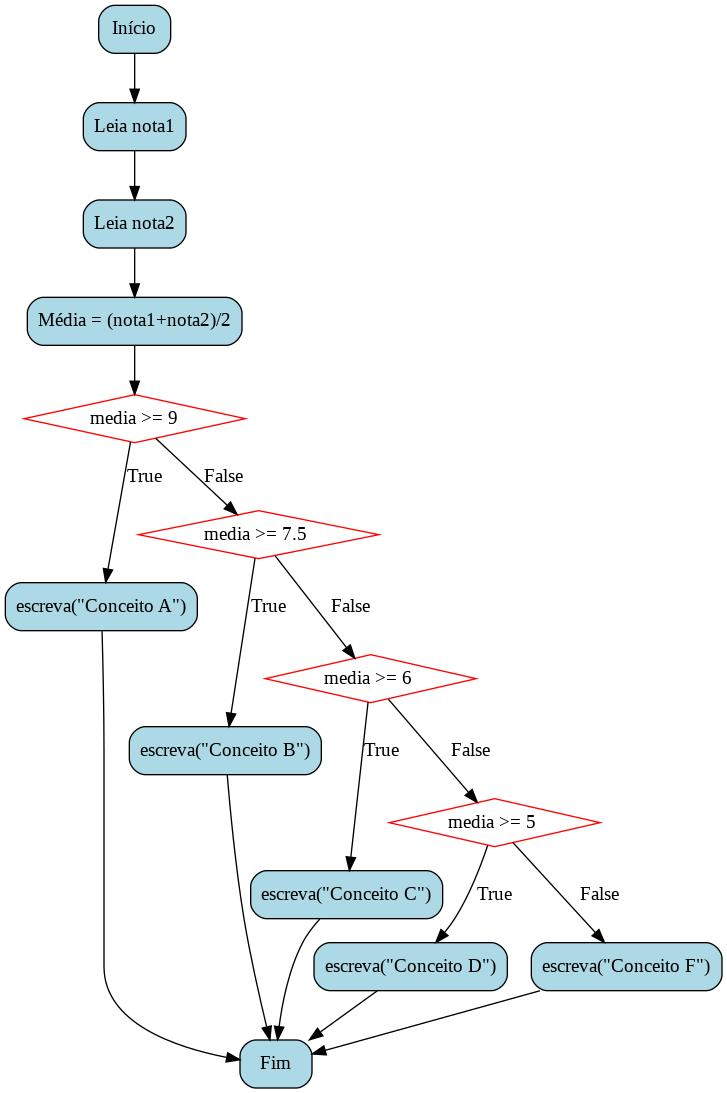
\includegraphics{"figs/flowchartCap3b.jpg"}

    \begin{figure}
\centering
\caption{flowchartCap3b.jpg}
\end{figure}

    \begin{tcolorbox}[breakable, size=fbox, boxrule=1pt, pad at break*=1mm,colback=cellbackground, colframe=cellborder]
\prompt{In}{incolor}{ }{\boxspacing}
\begin{Verbatim}[commandchars=\\\{\}]
\PY{k+kn}{from} \PY{n+nn}{txtoflow} \PY{k+kn}{import} \PY{n}{txtoflow}

\PY{n}{txtoflow}\PY{o}{.}\PY{n}{generate}\PY{p}{(}
    \PY{l+s+sd}{\PYZsq{}\PYZsq{}\PYZsq{}}
\PY{l+s+sd}{    Início;}
\PY{l+s+sd}{    Leia nota1;}
\PY{l+s+sd}{    Leia nota2;}
\PY{l+s+sd}{    Média = (nota1+nota2)/2;}
\PY{l+s+sd}{    if ( media \PYZgt{}= 9 ) \PYZob{}}
\PY{l+s+sd}{        escreva(\PYZdq{}Conceito A\PYZdq{}); }
\PY{l+s+sd}{    \PYZcb{} else if (media \PYZgt{}= 7.5 ) \PYZob{}}
\PY{l+s+sd}{        escreva(\PYZdq{}Conceito B\PYZdq{}); }
\PY{l+s+sd}{    \PYZcb{} else if (media \PYZgt{}= 6 ) \PYZob{}}
\PY{l+s+sd}{        escreva(\PYZdq{}Conceito C\PYZdq{}); }
\PY{l+s+sd}{    \PYZcb{} else if (media \PYZgt{}= 5 ) \PYZob{}}
\PY{l+s+sd}{        escreva(\PYZdq{}Conceito D\PYZdq{}); }
\PY{l+s+sd}{    \PYZcb{} else \PYZob{}}
\PY{l+s+sd}{        escreva(\PYZdq{}Conceito F\PYZdq{}); }
\PY{l+s+sd}{    \PYZcb{}}
\PY{l+s+sd}{    Fim;}
\PY{l+s+sd}{    \PYZsq{}\PYZsq{}\PYZsq{}}
\PY{p}{)}
\end{Verbatim}
\end{tcolorbox}

    Casos para Teste Moodle+VPL

Para o professor criar uma atividade VPL no Moodle para este Exemplo 02,
basta incluir em \texttt{Casos\ para\ teste}, o seguinte texto (pode
incluir mais casos):

\begin{verbatim}
case=caso1
input=4.0
6.0
output= 
Conceito D
case=caso2
input=4.0
5.0
output= 
Conceito F
case=caso2
input=5.0
7.0
output= 
Conceito C
case=caso3
input=6.0
9.0
output= 
Conceito B
case=caso4
input=9.0
10.0
output= 
Conceito A
\end{verbatim}

    \begin{tcolorbox}[breakable, size=fbox, boxrule=1pt, pad at break*=1mm,colback=cellbackground, colframe=cellborder]
\prompt{In}{incolor}{ }{\boxspacing}
\begin{Verbatim}[commandchars=\\\{\}]
\PY{o}{\PYZpc{}\PYZpc{}writefile} cap03exem02.c
\PY{c+c1}{\PYZsh{}include \PYZlt{}stdio.h\PYZgt{}}
\PY{n+nb}{float} \PY{n}{leia}\PY{p}{(}\PY{p}{)} \PY{p}{\PYZob{}}
  \PY{n+nb}{float} \PY{n}{valor}\PY{p}{;}
  \PY{n}{printf}\PY{p}{(}\PY{l+s+s2}{\PYZdq{}}\PY{l+s+s2}{Entre com um valor: }\PY{l+s+s2}{\PYZdq{}}\PY{p}{)}\PY{p}{;}
  \PY{n}{scanf}\PY{p}{(}\PY{l+s+s2}{\PYZdq{}}\PY{l+s+si}{\PYZpc{}f}\PY{l+s+s2}{\PYZdq{}}\PY{p}{,} \PY{o}{\PYZam{}}\PY{n}{valor}\PY{p}{)}\PY{p}{;}
  \PY{k}{return} \PY{n}{valor}\PY{p}{;}
\PY{p}{\PYZcb{}}

\PY{n+nb}{int} \PY{n}{main}\PY{p}{(}\PY{n}{void}\PY{p}{)} \PY{p}{\PYZob{}}

  \PY{o}{/}\PY{o}{/} \PY{n}{ENTRADAS}
  \PY{n+nb}{float} \PY{n}{nota1} \PY{o}{=} \PY{n}{leia}\PY{p}{(}\PY{p}{)}\PY{p}{;}
  \PY{n+nb}{float} \PY{n}{nota2} \PY{o}{=} \PY{n}{leia}\PY{p}{(}\PY{p}{)}\PY{p}{;}

  \PY{o}{/}\PY{o}{/} \PY{n}{PROCESSAMENTO} \PY{n}{E} \PY{n}{SAÍDA}
  \PY{n+nb}{float} \PY{n}{media} \PY{o}{=} \PY{p}{(}\PY{n}{nota1} \PY{o}{+} \PY{n}{nota2}\PY{p}{)}\PY{o}{/}\PY{l+m+mi}{2}\PY{p}{;}
  \PY{k}{if} \PY{p}{(}\PY{n}{media} \PY{o}{\PYZgt{}}\PY{o}{=} \PY{l+m+mf}{9.0}\PY{p}{)}      
    \PY{n}{printf}\PY{p}{(}\PY{l+s+s2}{\PYZdq{}}\PY{l+s+s2}{Conceito A}\PY{l+s+s2}{\PYZdq{}}\PY{p}{)}\PY{p}{;} 
  \PY{k}{else} \PY{k}{if} \PY{p}{(}\PY{n}{media} \PY{o}{\PYZgt{}}\PY{o}{=} \PY{l+m+mf}{7.5}\PY{p}{)} 
    \PY{n}{printf}\PY{p}{(}\PY{l+s+s2}{\PYZdq{}}\PY{l+s+s2}{Conceito B}\PY{l+s+s2}{\PYZdq{}}\PY{p}{)}\PY{p}{;}
  \PY{k}{else} \PY{k}{if} \PY{p}{(}\PY{n}{media} \PY{o}{\PYZgt{}}\PY{o}{=} \PY{l+m+mf}{6.0}\PY{p}{)} 
    \PY{n}{printf}\PY{p}{(}\PY{l+s+s2}{\PYZdq{}}\PY{l+s+s2}{Conceito C}\PY{l+s+s2}{\PYZdq{}}\PY{p}{)}\PY{p}{;}
  \PY{k}{else} \PY{k}{if} \PY{p}{(}\PY{n}{media} \PY{o}{\PYZgt{}}\PY{o}{=} \PY{l+m+mf}{5.0}\PY{p}{)} 
    \PY{n}{printf}\PY{p}{(}\PY{l+s+s2}{\PYZdq{}}\PY{l+s+s2}{Conceito D}\PY{l+s+s2}{\PYZdq{}}\PY{p}{)}\PY{p}{;}
  \PY{k}{else}        
    \PY{n}{printf}\PY{p}{(}\PY{l+s+s2}{\PYZdq{}}\PY{l+s+s2}{Reprovado! Conceito F.}\PY{l+s+s2}{\PYZdq{}}\PY{p}{)}\PY{p}{;}
  \PY{k}{return} \PY{l+m+mi}{0}\PY{p}{;}
\PY{p}{\PYZcb{}}
\end{Verbatim}
\end{tcolorbox}

    \begin{tcolorbox}[breakable, size=fbox, boxrule=1pt, pad at break*=1mm,colback=cellbackground, colframe=cellborder]
\prompt{In}{incolor}{ }{\boxspacing}
\begin{Verbatim}[commandchars=\\\{\}]
\PY{o}{\PYZpc{}\PYZpc{}}\PY{k}{shell}
gcc cap03exem02.c \PYZhy{}o output2
./output2
\end{Verbatim}
\end{tcolorbox}

    \hypertarget{exercuxedcios}{%
\subsection{Exercícios}\label{exercuxedcios}}

    Ver notebook Colab no arquivo \texttt{cap03.part2.lab.*.ipynb}
(\texttt{*} é a extensão da linguagem), utilizando aluma linguagem de
programação de sua preferência, onganizadas em subpastas contidas de
\texttt{"gen"}, na pasta do Google Drive
\href{https://drive.google.com/drive/folders/1YlFwv8XYN7PYYf-HwDMlkxzbmXzJw9cM?usp=sharing}{colabs}.

    \hypertarget{revisuxe3o-deste-capuxedtulo-de-desvios-condicionais}{%
\subsection{Revisão deste capítulo de Desvios
Condicionais}\label{revisuxe3o-deste-capuxedtulo-de-desvios-condicionais}}

\begin{itemize}
\tightlist
\item
  O que é um desvio condicional?
\item
  Condições com lógica booleana
\item
  Desvios condicionais Simples e Compostos, com Encadeamentos
\item
  Exercícios
\item
  Revisão deste capítulo de Desvios Condicionais
\end{itemize}


    % Add a bibliography block to the postdoc
    
    
    
\end{document}
